\documentclass[12pt]{article}
\usepackage[ansinew]{inputenc} % ASCII (Western CP)
\usepackage{graphicx}
\usepackage{color}
\usepackage[colorlinks]{hyperref}
\usepackage{geometry}
\geometry{left=2.5cm,right=2.5cm,top=2.5cm,bottom=2.5cm}

\title{Colinear Convolution Layer}
\author{Pang Liang}

\begin{document}
\maketitle

\section{Cifar10 Database}
The CIFAR-10 dataset consists of 60000 32x32 colour images in 10 classes, with 6000 images per class. There are 50000 training images and 10000 test images. (See \url{http://www.cs.toronto.edu/~kriz/cifar.html})

Fig~\ref{fig:cifar10} are the classes in the dataset, as well as 10 random images from each.
\begin{figure}[!ht]
    \centering
    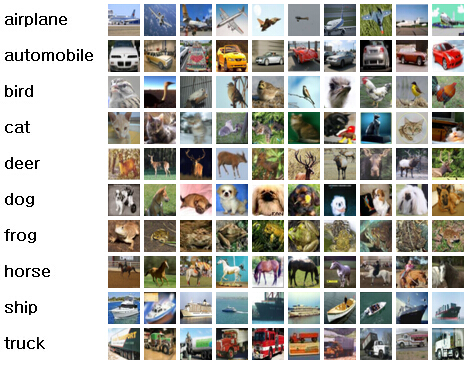
\includegraphics[height=8cm]{sample.jpg}
    \caption{\label{fig:cifar10} Example of cifar10 database. }
\end{figure}

\section{Caffe Framework of Deep Learning}
Caffe is a deep learning framework developed with cleanliness, readability, and speed in mind. (See \url{http://caffe.berkeleyvision.org})

It implement many kind of layers list below:
\begin{itemize}
    \item Vision Layers
    \begin{itemize}
        \item Convolution $\surd$
        \item Pooling $\surd$
        \item Local Response Normalization (LRN) $\surd$
    \end{itemize}
    \item Loss Layers
    \begin{itemize}
        \item Softmax $\surd$
        \item Sum-of-Squares / Euclidean
        \item Hinge / Margin
        \item Sigmoid Cross-Entropy
    %     \item Infogain
    %     \item Accuracy and Top-k
    \end{itemize}
    \item Activation / Neuron Layers
    \begin{itemize}
        \item ReLU / Rectified-Linear and Leaky-ReLU $\surd$
        \item Sigmoid
        \item TanH / Hyperbolic Tangent
    %     \item Absolute Value
    %     \item Power
    %     \item BNLL
    \end{itemize}
    % \item Data Layers
    % \begin{itemize}
    %     \item Database
    %     \item In-Memory
    %     \item HDF5 Input/HDF5 Output
    %     \item Images
    %     \item Windows
    %     \item Dummy
    % \end{itemize}
    \item Common Layers
    \begin{itemize}
        \item Inner Product $\surd$
        \item Splitting
        \item Flattening
        \item Concatenation
        \item Slicing
    \end{itemize}
\end{itemize}

\section{Fast Version of NN Structure for Cifar10}
The Cifar10 model Fig~\ref{fig:quick_model} is a CNN that composes layers of convolution, pooling, rectified linear unit (ReLU) nonlinearities, and local contrast normalization with a linear classifier on top of it all.

The inputs of the model are not the raw images or raw images normalized into $[0,1]$, but the images preprocess by the image mean operation. In other word, the pixel at same position average over all images, so the input pixel value range is $[-127,127]$. In the end of the network we use Softmax loss as the classification loss.

\begin{figure}[!ht]
    \centering
    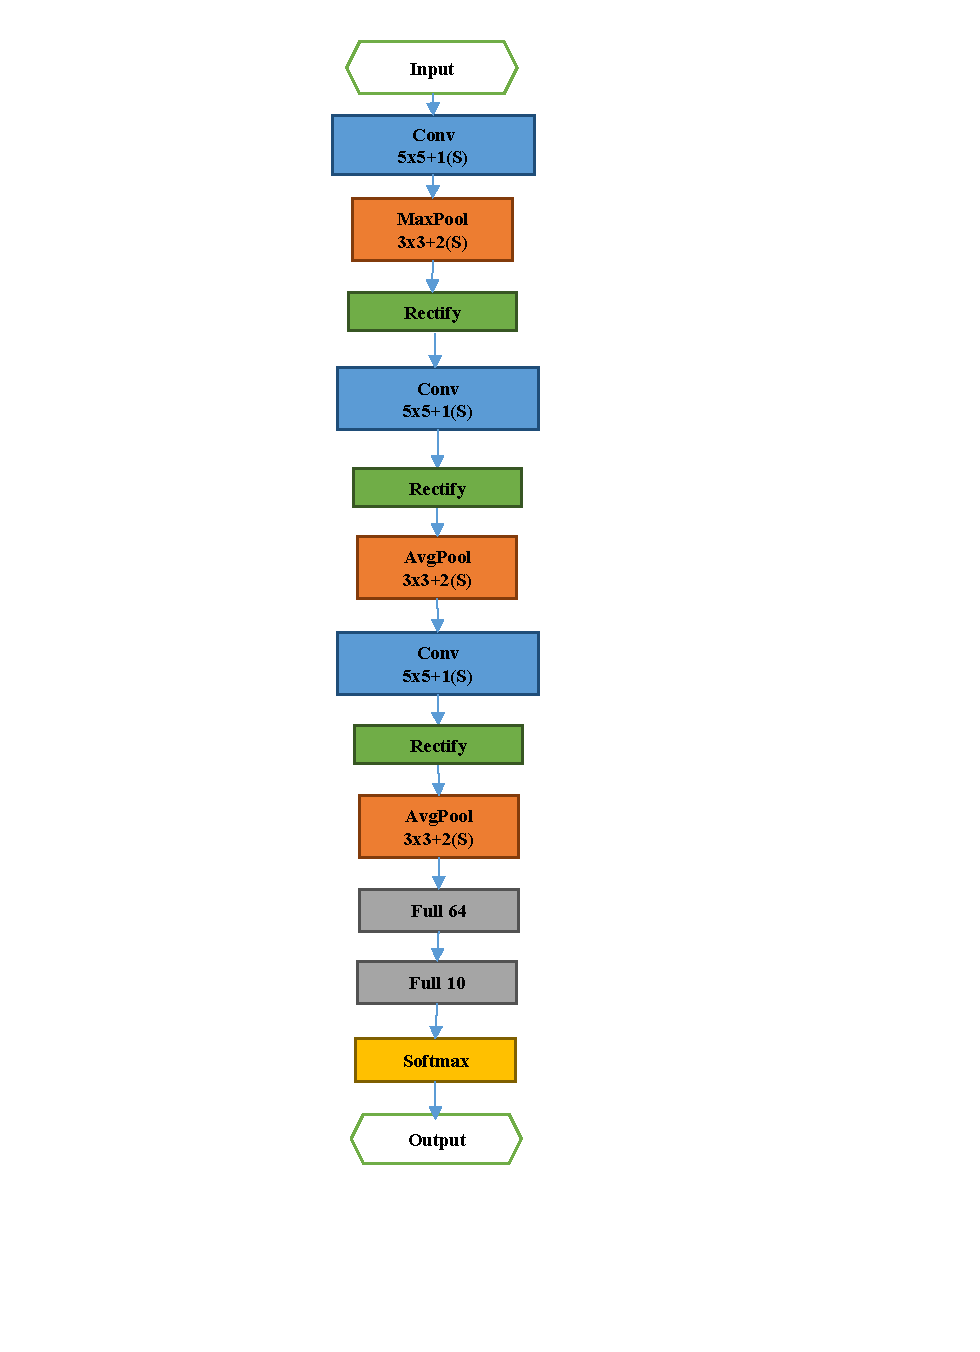
\includegraphics[height=15cm]{3.pdf}
    \caption{\label{fig:quick_model} Cifar10 quick model. }
\end{figure}

\section{Compare to Other Method}
    \subsection{Network in Network}
    
    For more detail of the caffe configuration of NIN(CCCP Layer), see \url{https://gist.github.com/mavenlin/e56253735ef32c3c296d}.
    \subsection{Drop Connection}
    
    \subsection{GoogLeNet 2014}

\section{Colinear Convolution Layer in Formula}
    \subsection{Feed Forward}
    \begin{equation}
    \begin{array}{l}
    a_{in} = e_iF_ne_i^T + S_ne_i^T + b_n \\
    = \sum_x \sum_y e_{ix}f_{xyn}e_{iy} + \sum_x s_{xn}e_{ix} + b_n
    \end{array}
    \end{equation}

    \subsection{Back Propagation}
    \begin{equation}
    \sum_n \frac{\partial E}{\partial a_{in}} = \epsilon_{in}
    \end{equation}
    \begin{itemize}
        \item Error Propagation
        \begin{equation}
        \frac{\partial E}{\partial e_{ix}} = \sum_n \frac{\partial E}{\partial a_{in}} \cdot \frac{\partial a_{in}}{\partial e_{ix}} = \sum_n  \epsilon_{in} ((\sum_y (f_{xyn} + f_{yxn}) e_{iy}) + s_{xn})
        \end{equation}

        \item Weight Update
        \begin{equation}
        \frac{\partial E}{\partial f_{xyn}} = \sum_i \frac{\partial E}{\partial a_{in}} \cdot \frac{\partial a_{in}}{\partial f_{xyn}} = \sum_i  \epsilon_{in} e_{ix} e_{iy}
        \end{equation}
        \begin{equation}
        \frac{\partial E}{\partial s_{xn}} = \sum_i \frac{\partial E}{\partial a_{in}} \cdot \frac{\partial a_{in}}{\partial s_{xn}} = \sum_i  \epsilon_{in} e_{ix}
        \end{equation}
        \begin{equation}
        \frac{\partial E}{\partial b_n} = \sum_i \frac{\partial E}{\partial a_{in}} \cdot \frac{\partial a_{in}}{\partial b_n} = \sum_i  \epsilon_{in}
        \end{equation}
    \end{itemize}

    See details in Fig~\ref{fig:ccnn}.
    \begin{figure}[!ht]
        \centering
        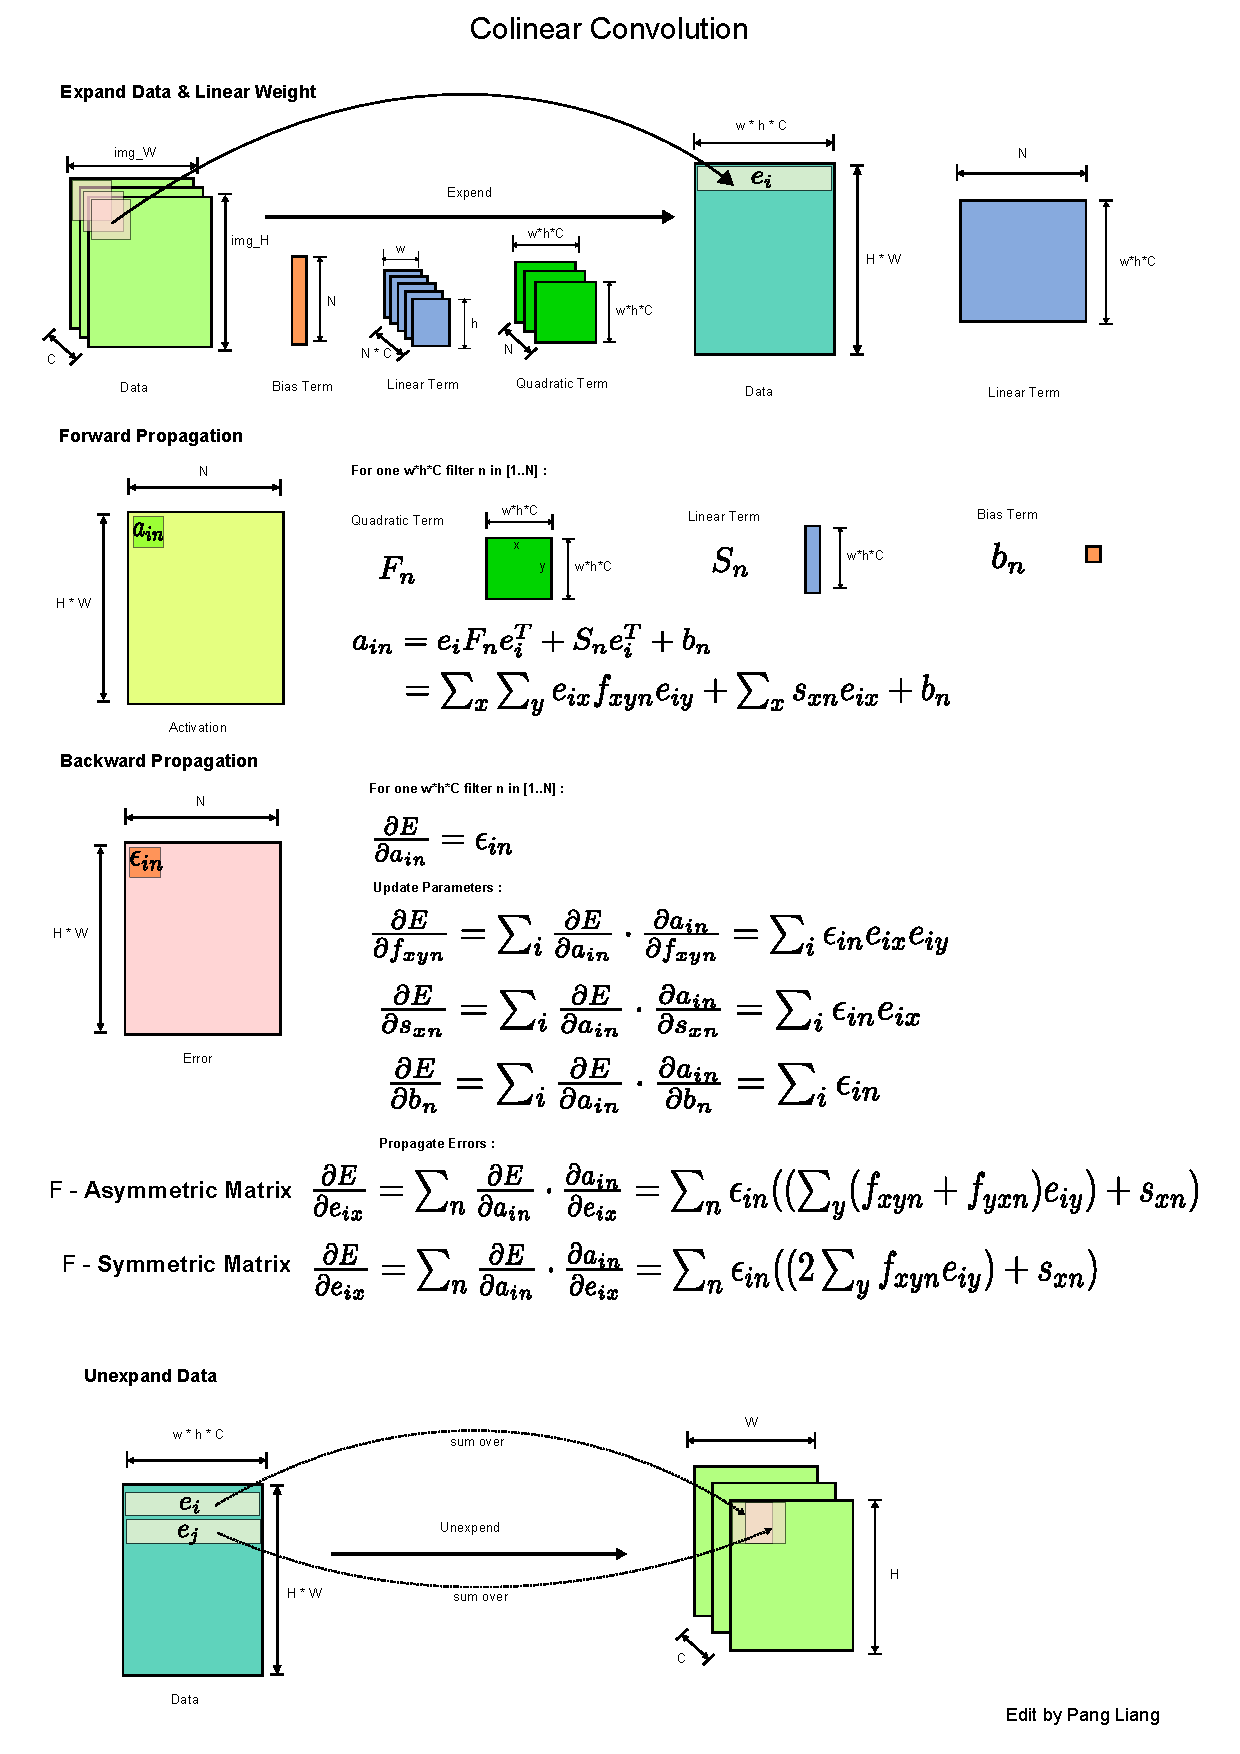
\includegraphics[height=18cm]{colinearcnn.pdf}
        \caption{\label{fig:ccnn} Colinear Convolution Layer.}
    \end{figure}

\section{Experiments}
We replace the first Convolution layer to our Colinear Convolution layer. Weights in quadratic term are initialed in range of $[0,0.000001]$, for the sake of the input range $[-127. 127]$ and form of $e*f*e$. We want the activations of the layer not too large, so the weights in quadratic term are very small. For the same reason, the weight decay is set to 1000.

In Fig~\ref{fig:loss} and Fig~\ref{fig:acc} ,the number 16 or 32 denotes the first convolution layer output channel number. The lines entitled with Base mean that the result produce by Convolution layer, and others without produce by Colinear Convolution layer. The experiments show that the original configuration of the network is better than what we proposed.But there're some points we should optimize, which will show in next section.
\begin{figure}[!ht]
    \centering
    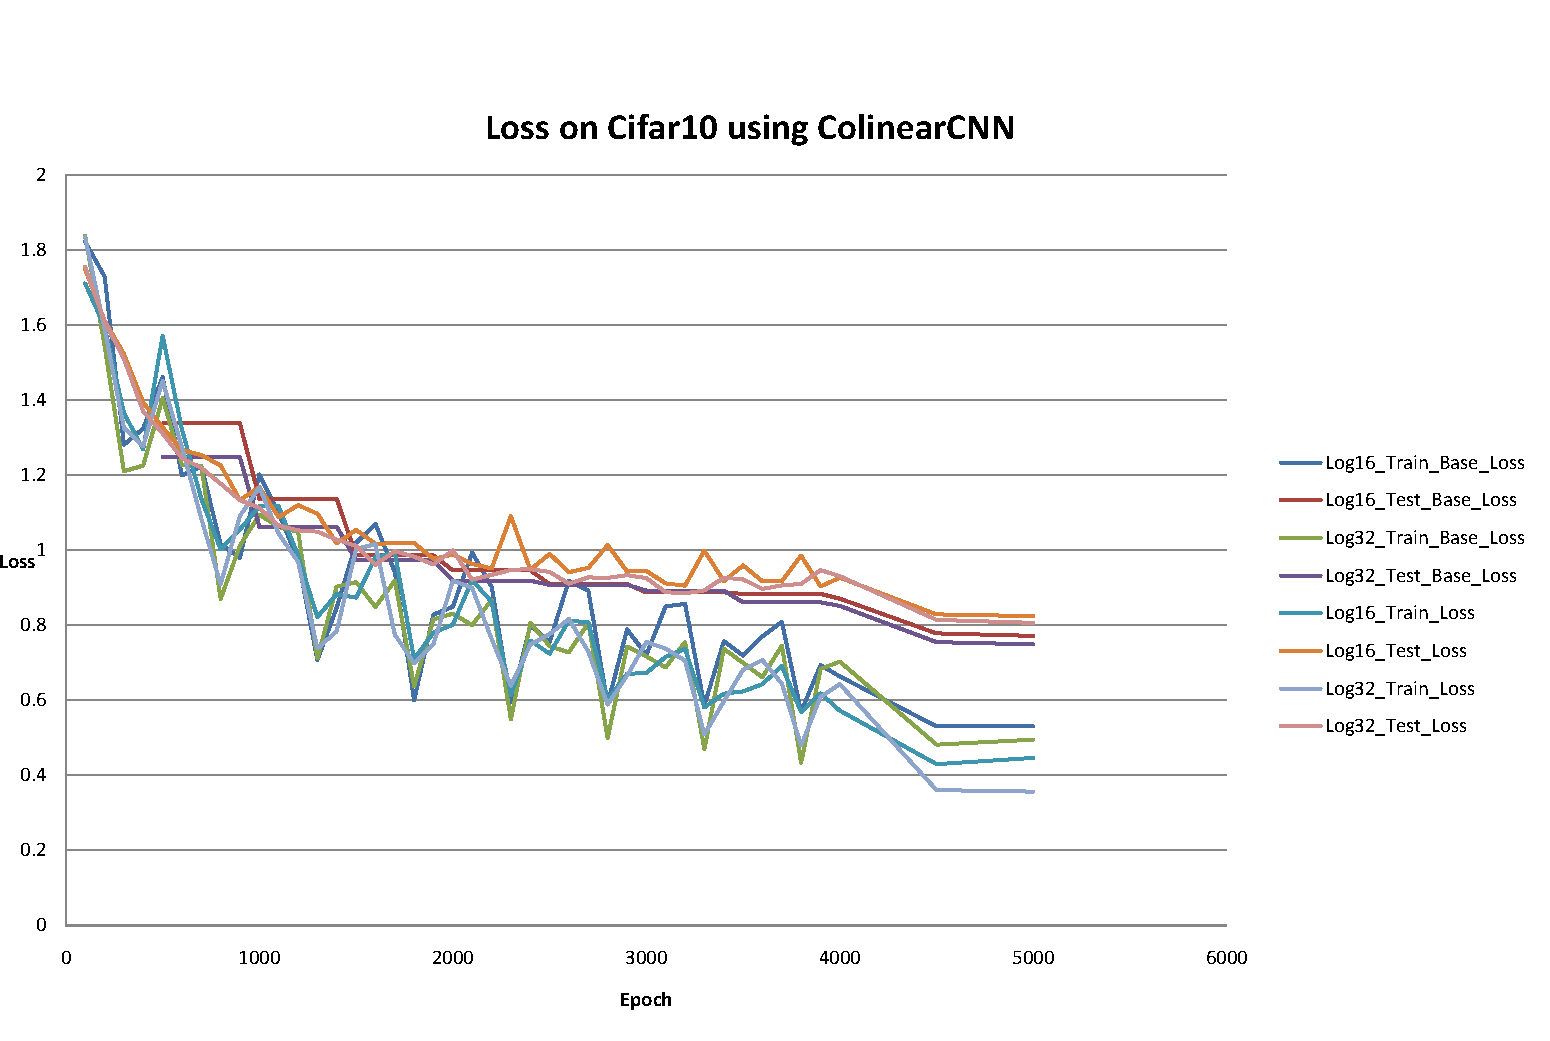
\includegraphics[height=10cm]{1.pdf}
    \caption{\label{fig:loss} Train loss and Test loss of four net structures.}
\end{figure}
\begin{figure}[!ht]
    \centering
    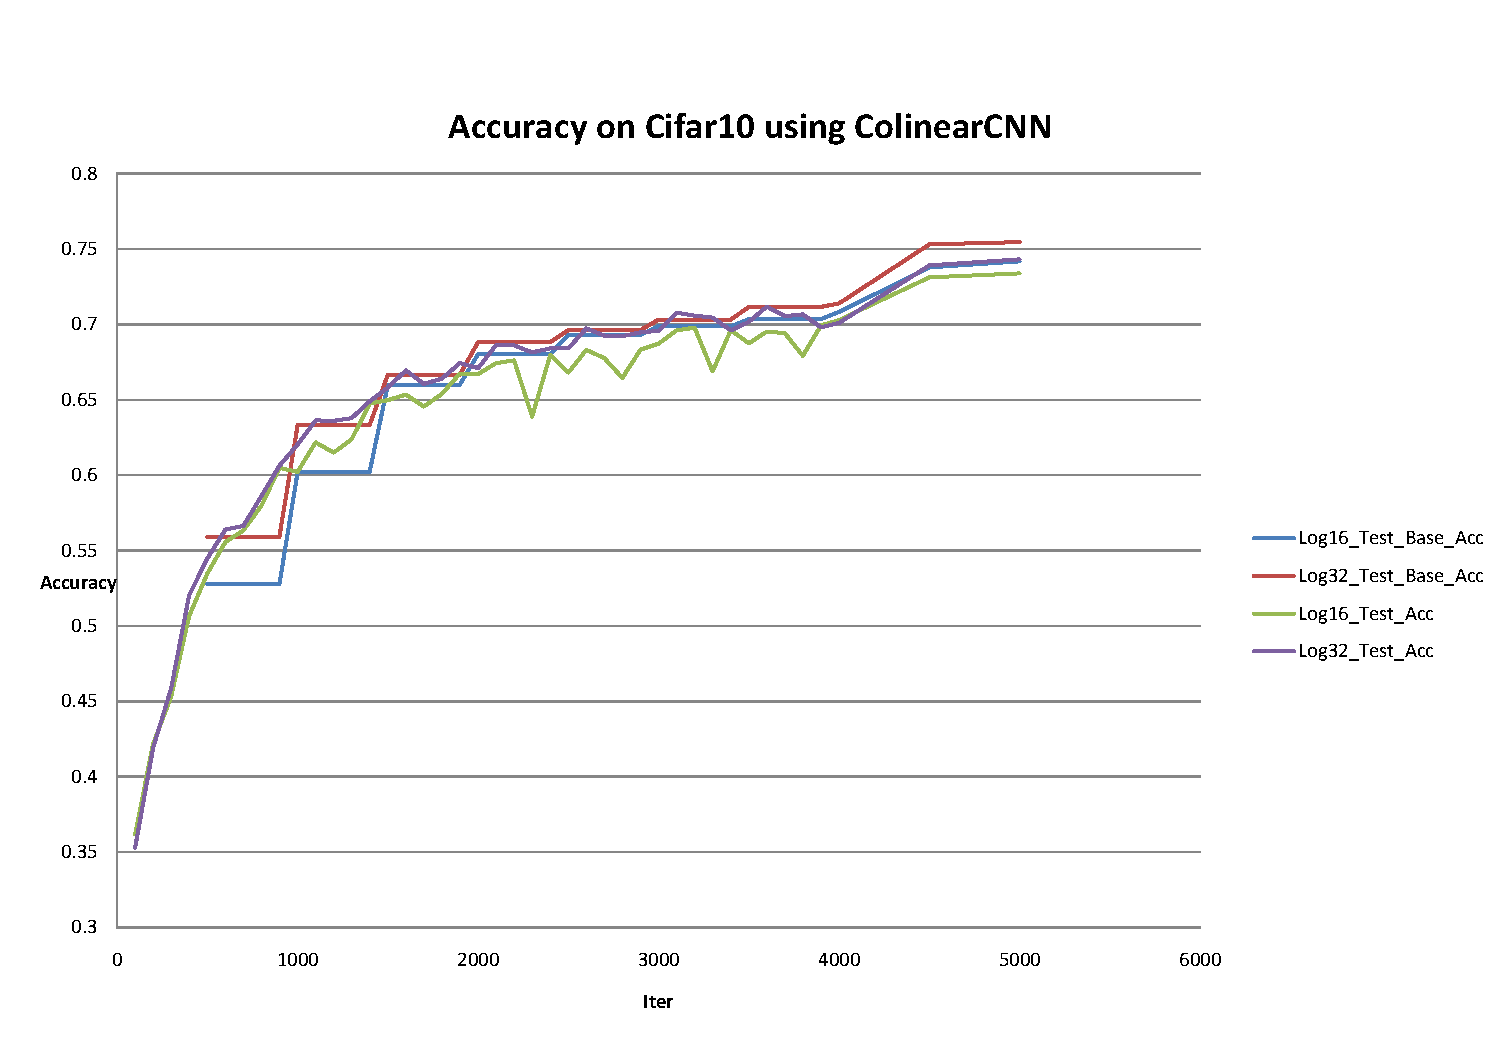
\includegraphics[height=10cm]{2.pdf}
    \caption{\label{fig:acc} Test Accuracy of four net structures.}
\end{figure}

\section{L1 Regularize on CCNN}
Using L1 regularize on the parameters always produces a more sparse result, which meanings the bigger the regularizer $\alpha$ the more 0 in parameters. Different from the L2 regularize $\lambda || W ||_2$, L1 regularize has the form of $\alpha || W ||_1$. L2 regularize can derived everywhere, see Eq~\ref{eq.l2}.
\begin{equation}
\frac{\partial{\lambda || W ||_2}}{\partial W} = 2 \lambda W \label{eq.l2}
\end{equation}

While L1 doesn't has this good property. Its derivative is Eq~\ref{eq.l1}.

\begin{equation}
\frac{\partial{\alpha || W ||_1}}{\partial W} = \left \{
\begin{array}{ll}
-\alpha & W<0 \\
undefine & W=0 \\
\alpha & W
\end{array} \right . \label{eq.l1}
\end{equation}

So in order to implement L1 regularize, we need to know $W$'s sign. For instance one parameter $w_t$ at $t$'s iterator, then we want to calculate next update of $w_t$ denoted as $w_{t+1}$.

\begin{equation}
w_{t+1} = w_t + \Delta w - sign(w) \alpha
\end{equation}

\begin{equation}
\hat{w_{t+1}} = w_t + \Delta w
\end{equation}

then we need $w_{t+1}$ and $w_t + \Delta w$ have the same sign. So the last term $-sign(w) \alpha$ will not change the sign. So we use Eq~\ref{eq.l1imp} for implement.

\begin{equation}
w_{t+1} = \left \{
\begin{array}{ll}
max(\hat{w_{t+1}}-\alpha, 0) & \hat{w_{t+1}}>=0 \\
min(\hat{w_{t+1}}+\alpha, 0) & \hat{w_{t+1}}<0
\end{array}
\right .
\label{eq.l1imp}
\end{equation}

\section{Symmetric Strategy on CCNN}
Changing Asymmetric Matrix $F$ to Symmetric Matrix is natural to us, because the relation between $e_{ix}$ and $e_{iy}$ should be same. That means $f_{xyn}=f_{yxn}$. So we decrease parameter number from $N^2$ to $N*(N+1)/2$.

Then we need modify some formula in BP process.
\begin{itemize}
    \item Error Propagation
    \begin{equation}
    \frac{\partial E}{\partial e_{ix}} = \sum_n \frac{\partial E}{\partial a_{in}} \cdot \frac{\partial a_{in}}{\partial e_{ix}} = \sum_n  \epsilon_{in} ((\sum_y 2 \cdot
    \left \{
        \begin{array}{ll}
        f_{xyn} & x<=y \\
        f_{yxn} & x>y
        \end{array}
    \right \}
    \cdot e_{iy}) + s_{xn})
    \end{equation}

    \item Weight Update
    \begin{equation}
    \frac{\partial E}{\partial f_{xyn}} = \sum_i \frac{\partial E}{\partial a_{in}} \cdot \frac{\partial a_{in}}{\partial f_{xyn}} =
    \left \{
        \begin{array}{ll}
        2 \sum_i  \epsilon_{in} e_{ix} e_{iy} & x<y \\
        \sum_i  \epsilon_{in} e_{ix} e_{iy} & x=y
        \end{array}
    \right .
    \end{equation}

\end{itemize}

\section{Mask the Parameters}
Maybe this idea can be compared with dropout connections.

\section{Restriction and Regularization of CCNN}
\begin{enumerate}
    \item Change the Asymmetric to Symmetric, in order to decrease the parameter numbers.
    \item Change the L2 regularize to L1 regularize, for the 2 order relation is weaker than the 1 order relation and we need not that much parameters to model it.
    \item Using mask matrix to erase the relations cross the channels.
\end{enumerate}
\end{document}
